\documentclass{article}
\usepackage{fullpage}
\usepackage{verbatim}
\usepackage{graphicx}
\usepackage{hyperref}
\usepackage{pdflscape}

\begin{document}
\setlength\parindent{0pt}
\section{Definition of Architecture}

First four definitions of software architecture are stated and their differences
and similarities are discussed. Second, our own view on software architecture is
given.
\subsection{Definitions on architectures}

\begin{enumerate}
\item Software Architecture is the set of structures needed to reason about the software system, which comprise the software elements, the relations between them, and the properties of both elements and relations.\cite{clemens}

\item Software Architecture is an abstract system specification consisting primarily of functional components described in terms of their behaviors and interfaces and component-component interconnections\cite{hayesroth}

\item Software Architecture is the fundamental organization of a system embodied in its components, their relationships to each other, and to the environment, and the principles guiding its design and evolution.\cite{IEEE1471}

\item Software architecture is the study of the large-scale structure and performance of software systems. Important aspects of a system's architecture include the division of functions among system modules, the means of communication between modules, and the representation of shared information.\cite{lane90}

\end{enumerate}

The definitions show a great deal of similarities. In all software architecture
is defined as a set of structures/components/modules, their properties and the
relationships between them. However each of the definitions highlights certain
aspects of architecture more than the others. 

\begin{itemize}
\item In \cite{clemens} and \cite{hayesroth} the focus has been put on the end result. The architecture is defined as the components themselves (their properties/interfaces) and the relationships between them (interconnections).
\item The definition stated in \cite{hayesroth} lays a focus on the functional components of a software architecture.
\item The definition of \cite{IEEE1471} is more focused around the process of
designing and maintaining an architecture. It explicitly states that the design
process and the evolution are part of the architecture itself.
\item The last definition (\cite{lane90}) focuses more on comparing
architectures and how the systems themselves perform. This also becomes clear
from the title of the article \emph{Studying Software Architecture Through
Design Spaces and Rules}.

\end{itemize}

\subsection{Our view on architecture}

We agree on the point that a software architecture is defined as a set of
structures, components and modules, their properties and the relations
between them. 
Not only we think it is important to let the architecture show the functional components, it might also be necessary to show some of the quality attributes that the stakeholders find important. \\ 

Our definition of software architecture will be:
Software architecture is the structure of a software system defining how it is
build up, which components it has and the relations between the components. 
A software architecture shows the functional and the quality requirements in
regard to the system.

%stakeholderpart
\section{Stakeholder Concerns}

In this project there are four different stakeholder :
\begin{enumerate}
\item The Initiator
\item AirFrance - KLM
\item The Dutch Government
\item EU Claim
\end{enumerate}

Each of them had different concerns within this project which are stated in the next subsections.

\subsection{Initiator}
The initiator is the one who started this project. He wants FlyWithUs to be a success and become the number one rating site people will go to. He want to be able to collect data from social media, other rating websites, news, weather and every other source that can be of importance. This data an then be used to provide the airlines with powerfull statistics and can give users a final rating. Users that make use of FlyWithUs have to be able to post reviews and ratings on the website and search for them. What makes FlyWithUs unique is the fact that airlines can get in touch with the users by sending them messages.

\subsection{AirFrance - KLM}
This stakeholder wants to have a reporting tool. With the tool he has to be able to see what recent reviews have been posted about his airline. Also, AirFrance - KLM wants to see statistics and be able to see what causes a sudden decline or increase in the rating. Furthermore, AirFrance-KLM wants to be able to enter flight information and by doing so influence the weight of review. This means that the weight of a rating has to be less when bad ratings are due to for example environmental issues (bad weather etc.) and have nothing to do with the airline companies services.

\subsection{Dutch Government}
Privacy is an important issue for the Dutch Government. The server needs to be hosted in the Netherlands so FlyWithUs will be led according to the Dutch Privacy Law. Also, the Dutch Governemnt would like to see the project to be a "Green IT" project. 

\subsection{EU Claim}
EU Claim wants to make certain that the privacy if the user is guaranteed. Furthermore the airlines have to behave on the website and do not mess with the results or bribe the users. Fairness is thus also an important issue to this stakeholder.

%Input viewpoints here
\section{Viewpoints}
% % % \input{PrivacyView}

\subsection{Privacy viewpoint}

\begin{itemize}
\item Related stakeholders: Dutch government, EU Claim
\item Related Concerns: Privacy of the user
\end{itemize}

\newpage
\begin{landscape}
\begin{figure}
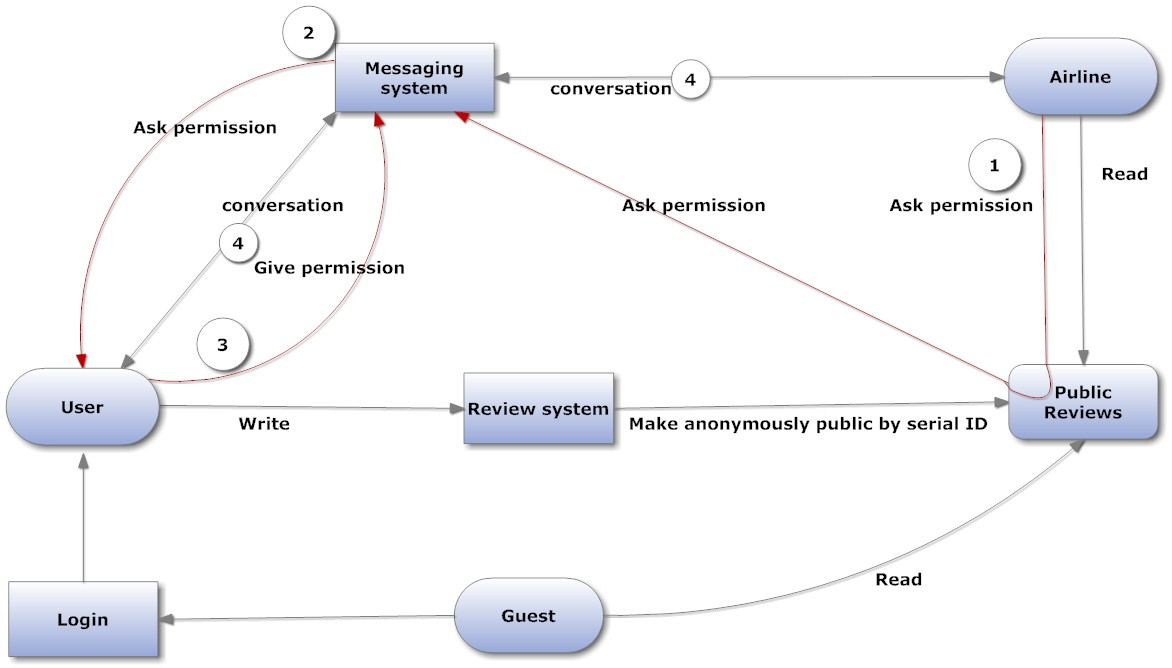
\includegraphics[width=680px]{privacyview}
\caption{Privacy viewpoint}
\label{fig:privacy}
\end{figure}
\end{landscape}
The privacy viewpoint in figure \ref{fig:privacy} shows how the privacy of the user is guaranteed in the system. A user can write a review that is shown to the public anonymously. The review will have a serialID instead of the user name so the user will stay unknown to the public. 

An airline should be able to have a conversation with an user if the airline wants to elaborate on a specific case or wants to adress the user personally. If the airline wants to get the user's information for a conversation it should ask permission of the user. When a user accepts to have a conversation with an airline the user's contact information is visible to the airline so they will be able to have a conversation. If the user is not satisfied with how the airline company responds on requests or remarks in the conversation, the user is able to invite EU Claim to the conversation so they will be able to see the conversation and decide to act upon it.

\subsection{Privacy viewpoint}

\begin{itemize}
\item Related stakeholders: Dutch government, EU Claim
\item Related Concerns: Privacy of the user
\end{itemize}

\newpage
\begin{landscape}
\begin{figure}
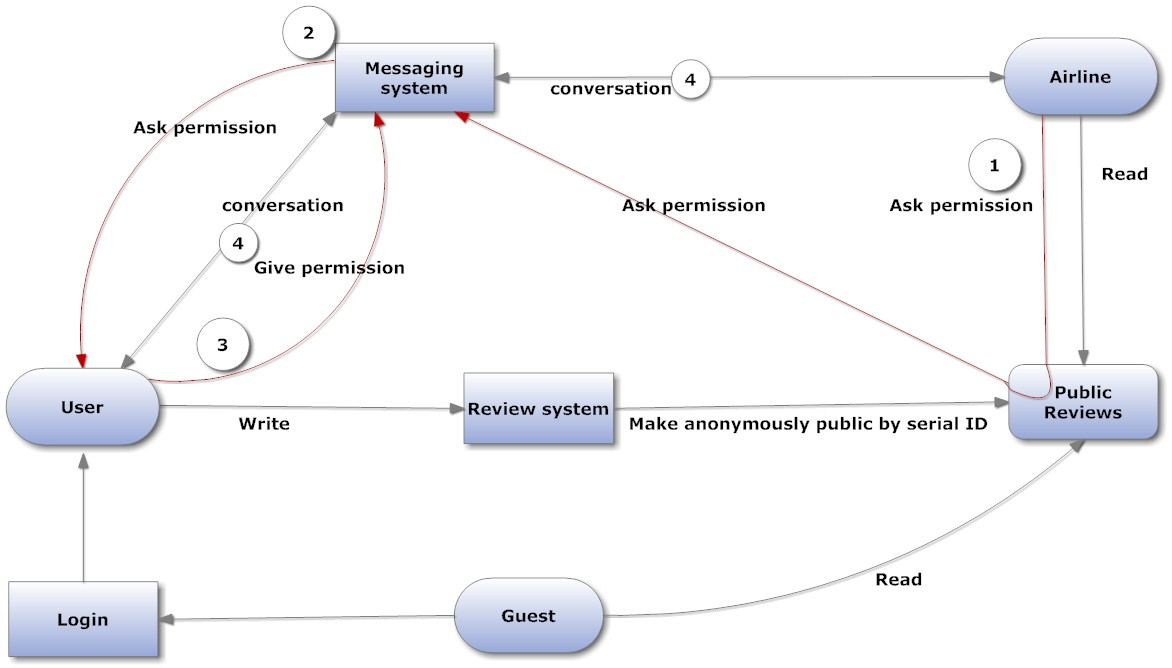
\includegraphics[width=680px]{privacyview}
\caption{Privacy viewpoint}
\label{fig:privacy}
\end{figure}
\end{landscape}
The privacy viewpoint in figure \ref{fig:privacy} shows how the privacy of the user is guaranteed in the system. A user can write a review that is shown to the public anonymously. The review will have a serialID instead of the user name so the user will stay unknown to the public. 

An airline should be able to have a conversation with an user if the airline wants to elaborate on a specific case or wants to adress the user personally. If the airline wants to get the user's information for a conversation it should ask permission of the user. When a user accepts to have a conversation with an airline the user's contact information is visible to the airline so they will be able to have a conversation. If the user is not satisfied with how the airline company responds on requests or remarks in the conversation, the user is able to invite EU Claim to the conversation so they will be able to see the conversation and decide to act upon it.

\subsection{Privacy viewpoint}

\begin{itemize}
\item Related stakeholders: Dutch government, EU Claim
\item Related Concerns: Privacy of the user
\end{itemize}

\newpage
\begin{landscape}
\begin{figure}
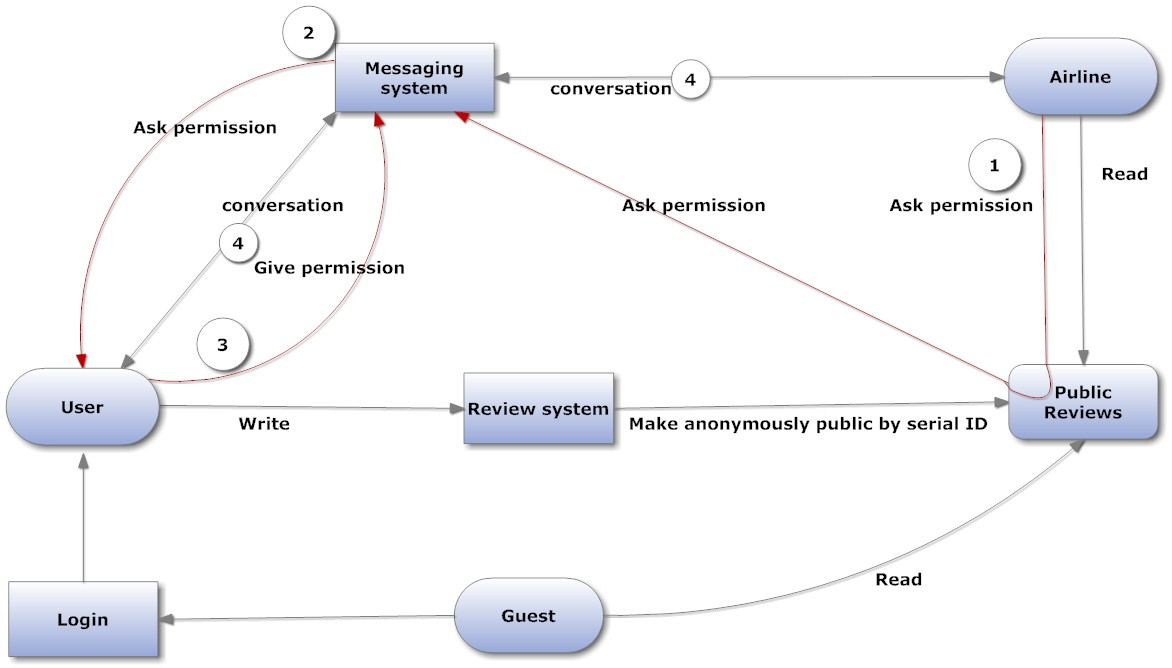
\includegraphics[width=680px]{privacyview}
\caption{Privacy viewpoint}
\label{fig:privacy}
\end{figure}
\end{landscape}
The privacy viewpoint in figure \ref{fig:privacy} shows how the privacy of the user is guaranteed in the system. A user can write a review that is shown to the public anonymously. The review will have a serialID instead of the user name so the user will stay unknown to the public. 

An airline should be able to have a conversation with an user if the airline wants to elaborate on a specific case or wants to adress the user personally. If the airline wants to get the user's information for a conversation it should ask permission of the user. When a user accepts to have a conversation with an airline the user's contact information is visible to the airline so they will be able to have a conversation. If the user is not satisfied with how the airline company responds on requests or remarks in the conversation, the user is able to invite EU Claim to the conversation so they will be able to see the conversation and decide to act upon it.


\section{Description of our Solution}

\appendix

\section{Domain Knowledge - Design Decision}
In this section we will present the domain specific problems related to airline reputation management system. To divide the workload four separate directions were defined. These  
directions are highly interconnected and might not appear as separate in the final design. The four directions are:
\begin{enumerate}
\item User Experience
\item Competition and Functionality
\item Data storage
\item Data Gathering
\end{enumerate}
A separate section has been dedicated to each of the direction. 

\subsection{Domain Specific Problems Related to User Experience}
\subsubsection{Important Questions}
The purpose of this section is to ask domain specific question related to user experience. The interface consists of all front-end systems that are directly in contact with the users. 
In order to get a better insight over the domain we searched through websites relevant to airline companies. We tried to understand what is important to the users and what they are looking for in
a rating site. The questions that  are important to the interfaces which affect user experience are:
\begin{enumerate}
\item What types of customers are distinguished in the system?
\item What kind of interactions should each customer be able to perform?
\end{enumerate}

\subsubsection{Design Decisions}
During our meetings with the stakeholders it was made clear that there are two types of customers:
\begin{enumerate} 
\item Clients: In general, the people who write and read the reviews and ratings.
\item Business Clients: The airline companies. The airline companies want to see a general overview of their companies ratings and reviews with some additional features such as the 
reporting system (discussed in the next section)
\end{enumerate}

An overview of the functionalities available to these groups of user is described below: 
\begin{itemize}
\item Clients (Registered Users):
	\begin{enumerate}
		\item They can write ({\em anonymously}), read and vote the reviews (Review System).
        \item They can see and compare the ratings of different airline companies.
        \item They can accept the invitation of an airline based on one of their reviews to a private conversation (Messaging System). 
		\item They can Invite EU claim to a private conversation.
	\end{enumerate}
\item Business Clients (Airline Companies):
	\begin{enumerate}
		\item They can write feedback to a user's review.
		\item They can invite a user to a private conversation based on a review in order to resolve his/ her complaint.
		\item They can see the current ratings and/ or the latest (bad) reviews posted (Reporting System).
		\item They can see statistics about their progress.
		\item They can see their progress in comparison with other airline's progress (only if they share their information as well).
		\item They can insert flight information and search through our databases to find patterns.
	\end{enumerate}
\end{itemize}

The fact that these two groups have clearly different functionalities results in two options concerning the system's interface, either two totally separate sites, or a general page 
whose content will change depending on the signed in user but the lay out will be the same.

In addition to these groups there two more:
\begin{itemize}
 \item Guests: Unregistered users who can only search for airlines and read reviews and ratings.
 \item EU-Claim: EU-Claim can monitor a private conversation after a user's invitation. Furthermore, is notified if a conversation is not ''resolved'' for a specified period of time.
\end{itemize}


\subsection{Domain Specific Problems Related to Competition and Functionality}
\subsubsection{Important Questions}
The purpose of this section is to find the domain specific questions related to our functionality. To accomplish that, we searched in the internet to learn more about our competition
and what they offer in order to adapt our system's architecture to focus on the functionalities that are going to differentiate us from them. The questions that help us understand the 
domain are:
\begin{enumerate}
\item Who is our biggest competitor?
\item Do we need to handle online payment?
\item How do the feedback and the messaging systems work?
\item How will the reporting system work?
\item How can we protect our results?
\item How do we ensure the users' privacy?
\item Which features of our review format are going to ensure users' privacy?
\end{enumerate}

\subsubsection{Design Decisions}
\paragraph{Competition} Our greatest competitor seems to be http://www.airlinequality.com/. This site contains reviews about 681 airlines and 725 airports and uses a “star” rating 
system called SKYTRAX. SKYTRAX has been used since 1999 and right now seems to be the only globally accepted airline rating system (is recognized as a global benchmark for airline 
standards). Fortunately, it does not provide feedback and reporting system. Consequently it is recommended to focus these systems.

\paragraph{Online Payment} It was requested that the services to the airlines will be available after payment. The payment can either take place online or offline. In the first case, 
the stakeholders are going to have an extra cost (fee: a percent of every transaction or predefined + 10\$ – 25\$ every month). On the other hand since the 
payment is addressed only to airline companies it is possible to do that offline through contracts, invoices etc.

\paragraph{Feedback \& Messaging System} The platform of FlyWithUs provides to the airlines the opportunity to respond to a review if they believe it is necessary. (Feedback system)

Additionally, an airline will be able to invite a user to a private conversation based on bad review in order to address an issue or to try to compensate him/ her. The user can choose 
if he/ she wants to continue and if he/ she wishes to provide his/ her information.

It is also significant to decide whether preserving the integrity of the system's  messaging service is desirable. To accomplish that, EU-Claim could be able to monitor the private 
conversation. Although the user will be notified about this, it may still be against his/ her privacy. EU-Claim proposed this functionality to be available only if the user enables 
it and not by default and KLM representative and the initiator agreed as well.

Furthermore, it is desirable for such a conversation to have states for example “resolved”  and “pending”, then a user can change a its state from pending to resolved. As a result 
EU-Claim can be notified by the system if a report has been unresolved for a certain period of time.  Additionally, the state of a conversation allows us to calculate the resolved 
issues and include that result in our website in order to encourage people to use our system.

\paragraph{Reporting System} The reporting system is a functionality only available to airlines. Each airline will be able to monitor its rating status through a report webpage which will comprise of the following components:
\begin{itemize}
\item Analytics concerning its progress through graphs and diagrams.
\item Latest reviews or bad reviews from our site.
\item Crossreference flight information with the reviews stored on our system.
\item Comparison between airlines (only if the airline shares her information also)
\end{itemize}

\paragraph{Prevent Aggregation – Copyright} The copyright of the data that will be collected should be further investigated according to the policy of each source. If the legality of 
harvesting data from the other sources is resolved and even if the data gathered are public, the collection of the data on our system can be protected. This can be achieved because 
even though the data are public a collection of them is copyrightable. Additionally, we can use a file called robots.txt to prevent data aggregation from specific crawlers. However, 
the effectiveness of this file lies entirely on the crawlers because they can ignore the file. It appears that there are no architecture relevant questions on this question.

\paragraph{Users' Privacy} As it was mentioned in the section Feedback \& Messaging Systems, users' privacy is an important issue. This issue was raised by three of the stakeholders 
Dutch government, EU-Claim and the initiator. A user's data and conversations with airlines are private, this means that these information are available only after user authentication 
and in the case of the private conversation available only to the airline of interest (maybe to EU-Claim as well if the user requests that). 

\paragraph{Review's Format} Since user's privacy is a big issue the review's format should allow anonymity. This is accomplished by omitting the name, username or any other author 
identifier from the public representation of a review.

\subsection{Domain specific problems related to data gathering and Analysis}
\subsubsection{Import questions}
The purpose of this section is to explain domain related problems related with this task. The data gathering is responsible for polling external sources and providing the data to the storage system. This implicates two important question which are further elaborated next:
\begin{enumerate}
\item	How is the data from different external sources combined?
\item	How is the combined data used in order to obtain a rating?
\item	Is there any filtering process on the external data?
\end{enumerate}
The external sources vary from airline companies sites to review sites to social networks. These all have their own way of inputting a review. For instance, Twitter does not have any format related to the review and only consists of lines text, while review sites already have  a format in place that allows the user to rate some of the attributes (Food, timeliness, service etc.) on a given scale. The final application should be able to digest all these kinds of reviews and output the results on a scale . 
A separate , however still important, question relates to the quality of the data. The external sources may or may not have systems in place that assure the quality of a review. Since the data is not inspected 

\subsubsection{Design Decisions}

\paragraph{Combining external sources}
The sources have their own unique format as explained earlier in the document. If the system where to parse this into a general format information might get lost or lot's of information is undefined.
However the general format helps decrease the complexity of analysing, because that system does not need to account for all the unique formats. This decision requires further collaboration with the data storage
as that needs to be able to handle the data. 

\paragraph{Analysing external sources}
Not all external sources give a rating on a scale (e.g. Twitter) therefore these reviews need to be analyzed first in order to be usefull. There are multiple options available when analyzing these results:
\begin{enumerate}
\item Drop all reviews that have no rating attached to them. This would lead to a huge data loss, but decrease the complexity of the system. The ratings can then easily be combined by computing a weighted average (or by another formula) of the individual ratings.
\item Transform the reviews without ratings by performing a sentiment analysis. After the analysis the ratings can be combined the same as in the other option.
\end{enumerate}

\paragraph{Filtering}
Some reviews may not be considered usefull, because of certain properties. The system could apply some business rules in order to filter those reviews out. The business rules governing these reviews are however currently unknown. 


\begin{thebibliography}{9}

\bibitem{clemens}
Bass et al.
  \emph{Software Architecture in Practice}.
  Addison Wesley, Boston,
  3nd Edition,
  2012.

\bibitem{hayesroth}
 Hayes-Roth, F
 \emph{Architecture-Based Acquisition and Development of Software: Guidelines and Recommendations from the ARPA Domain-Specific
 Software Architecture (DSSA) Program},
 Teknowledge Federal Systems,
 1994

\bibitem{IEEE1471}
 IEEE Std 1471-2000,
 \emph{Recommended Practice for Architecture Description of Software-Intensive Systems},
 United States,
 2000

\bibitem{lane90}
  Lane, Thomas,
  \emph{Studying Software Architecture Through Design Spaces and Rules}.
  Software Engineering Institute, Carnegie Mellon University,
  1990.

\end{thebibliography}

\end{document}

